
%%%%%%%%%%%%%
% NON SUDDIVIDERE IL TESTO DELLA TESI IN PIU' FILE LATEX
% COMPILARE LA TESI USANDO QUESTO https://it.overleaf.com/project/5ed943b9487c28000198567aUNICO FILE DI ESEMPIO PER I CONTENUTI TESTUALI
%%%%%%%%%%%%%

\documentclass[12pt,a4paper,twoside,openright]{book}

\usepackage[utf8]{inputenc}
\usepackage[italian]{babel}
\usepackage[T1]{fontenc}

\usepackage{style/isi_style_lt}

\usepackage{amsmath,amsfonts,amssymb,amsthm}
\usepackage{caption}
\usepackage[usenames]{color}
\usepackage{enumerate}
\usepackage{fancyhdr}
\usepackage{fancyvrb}
\usepackage{float}
\usepackage{graphicx}
\usepackage{booktabs}
\usepackage{indentfirst}
\usepackage{listings}
\usepackage{marvosym}
\usepackage{multicol}
\usepackage{sectsty}
\usepackage{subcaption}
\usepackage{tocloft}
\usepackage{microtype}
\usepackage[table]{xcolor}
\usepackage{url}
\usepackage{hyperref}
\usepackage{adjustbox}



    \usepackage{adjustbox} % Used to constrain images to a maximum size 
    \usepackage{textcomp} % defines textquotesingle
    % Hack from http://tex.stackexchange.com/a/47451/13684:
    \AtBeginDocument{%
        \def\PYZsq{\textquotesingle}% Upright quotes in Pygmentized code
    }
    \usepackage{upquote} % Upright quotes for verbatim code
    \usepackage{eurosym} % defines \euro
    \usepackage[mathletters]{ucs} % Extended unicode (utf-8) support
    \usepackage{grffile} % extends the file name processing of package graphics 
                         % to support a larger range 
    \usepackage{longtable} % longtable support required by pandoc >1.10
    \usepackage{booktabs}  % table support for pandoc > 1.12.2
    \usepackage[inline]{enumitem} % IRkernel/repr support (it uses the enumerate* environment)
    \usepackage[normalem]{ulem} % ulem is needed to support strikethroughs (\sout)

    
    % Colors for the hyperref package
    \definecolor{urlcolor}{rgb}{0,.145,.698}
    \definecolor{linkcolor}{rgb}{.71,0.21,0.01}
    \definecolor{citecolor}{rgb}{.12,.54,.11}

    % ANSI colors
    \definecolor{ansi-black}{HTML}{3E424D}
    \definecolor{ansi-black-intense}{HTML}{282C36}
    \definecolor{ansi-red}{HTML}{E75C58}
    \definecolor{ansi-red-intense}{HTML}{B22B31}
    \definecolor{ansi-green}{HTML}{00A250}
    \definecolor{ansi-green-intense}{HTML}{007427}
    \definecolor{ansi-yellow}{HTML}{DDB62B}
    \definecolor{ansi-yellow-intense}{HTML}{B27D12}
    \definecolor{ansi-blue}{HTML}{208FFB}
    \definecolor{ansi-blue-intense}{HTML}{0065CA}
    \definecolor{ansi-magenta}{HTML}{D160C4}
    \definecolor{ansi-magenta-intense}{HTML}{A03196}
    \definecolor{ansi-cyan}{HTML}{60C6C8}
    \definecolor{ansi-cyan-intense}{HTML}{258F8F}
    \definecolor{ansi-white}{HTML}{C5C1B4}
    \definecolor{ansi-white-intense}{HTML}{A1A6B2}

    % commands and environments needed by pandoc snippets
    % extracted from the output of `pandoc -s`
    \providecommand{\tightlist}{%
      \setlength{\itemsep}{0pt}\setlength{\parskip}{0pt}}
    \DefineVerbatimEnvironment{Highlighting}{Verbatim}{commandchars=\\\{\}}
    % Add ',fontsize=\small' for more characters per line
    \newenvironment{Shaded}{}{}
    \newcommand{\KeywordTok}[1]{\textcolor[rgb]{0.00,0.44,0.13}{\textbf{{#1}}}}
    \newcommand{\DataTypeTok}[1]{\textcolor[rgb]{0.56,0.13,0.00}{{#1}}}
    \newcommand{\DecValTok}[1]{\textcolor[rgb]{0.25,0.63,0.44}{{#1}}}
    \newcommand{\BaseNTok}[1]{\textcolor[rgb]{0.25,0.63,0.44}{{#1}}}
    \newcommand{\FloatTok}[1]{\textcolor[rgb]{0.25,0.63,0.44}{{#1}}}
    \newcommand{\CharTok}[1]{\textcolor[rgb]{0.25,0.44,0.63}{{#1}}}
    \newcommand{\StringTok}[1]{\textcolor[rgb]{0.25,0.44,0.63}{{#1}}}
    \newcommand{\CommentTok}[1]{\textcolor[rgb]{0.38,0.63,0.69}{\textit{{#1}}}}
    \newcommand{\OtherTok}[1]{\textcolor[rgb]{0.00,0.44,0.13}{{#1}}}
    \newcommand{\AlertTok}[1]{\textcolor[rgb]{1.00,0.00,0.00}{\textbf{{#1}}}}
    \newcommand{\FunctionTok}[1]{\textcolor[rgb]{0.02,0.16,0.49}{{#1}}}
    \newcommand{\RegionMarkerTok}[1]{{#1}}
    \newcommand{\ErrorTok}[1]{\textcolor[rgb]{1.00,0.00,0.00}{\textbf{{#1}}}}
    \newcommand{\NormalTok}[1]{{#1}}
    
    % Additional commands for more recent versions of Pandoc
    \newcommand{\ConstantTok}[1]{\textcolor[rgb]{0.53,0.00,0.00}{{#1}}}
    \newcommand{\SpecialCharTok}[1]{\textcolor[rgb]{0.25,0.44,0.63}{{#1}}}
    \newcommand{\VerbatimStringTok}[1]{\textcolor[rgb]{0.25,0.44,0.63}{{#1}}}
    \newcommand{\SpecialStringTok}[1]{\textcolor[rgb]{0.73,0.40,0.53}{{#1}}}
    \newcommand{\ImportTok}[1]{{#1}}
    \newcommand{\DocumentationTok}[1]{\textcolor[rgb]{0.73,0.13,0.13}{\textit{{#1}}}}
    \newcommand{\AnnotationTok}[1]{\textcolor[rgb]{0.38,0.63,0.69}{\textbf{\textit{{#1}}}}}
    \newcommand{\CommentVarTok}[1]{\textcolor[rgb]{0.38,0.63,0.69}{\textbf{\textit{{#1}}}}}
    \newcommand{\VariableTok}[1]{\textcolor[rgb]{0.10,0.09,0.49}{{#1}}}
    \newcommand{\ControlFlowTok}[1]{\textcolor[rgb]{0.00,0.44,0.13}{\textbf{{#1}}}}
    \newcommand{\OperatorTok}[1]{\textcolor[rgb]{0.40,0.40,0.40}{{#1}}}
    \newcommand{\BuiltInTok}[1]{{#1}}
    \newcommand{\ExtensionTok}[1]{{#1}}
    \newcommand{\PreprocessorTok}[1]{\textcolor[rgb]{0.74,0.48,0.00}{{#1}}}
    \newcommand{\AttributeTok}[1]{\textcolor[rgb]{0.49,0.56,0.16}{{#1}}}
    \newcommand{\InformationTok}[1]{\textcolor[rgb]{0.38,0.63,0.69}{\textbf{\textit{{#1}}}}}
    \newcommand{\WarningTok}[1]{\textcolor[rgb]{0.38,0.63,0.69}{\textbf{\textit{{#1}}}}}
    
    
    % Define a nice break command that doesn't care if a line doesn't already
    % exist.
    \def\br{\hspace*{\fill} \\* }
    % Math Jax compatability definitions
    \def\gt{>}
    \def\lt{<}
    % Document parameters
    \title{Untitled1}
    
    
    

    % Pygments definitions
    
\makeatletter
\def\PY@reset{\let\PY@it=\relax \let\PY@bf=\relax%
    \let\PY@ul=\relax \let\PY@tc=\relax%
    \let\PY@bc=\relax \let\PY@ff=\relax}
\def\PY@tok#1{\csname PY@tok@#1\endcsname}
\def\PY@toks#1+{\ifx\relax#1\empty\else%
    \PY@tok{#1}\expandafter\PY@toks\fi}
\def\PY@do#1{\PY@bc{\PY@tc{\PY@ul{%
    \PY@it{\PY@bf{\PY@ff{#1}}}}}}}
\def\PY#1#2{\PY@reset\PY@toks#1+\relax+\PY@do{#2}}

\expandafter\def\csname PY@tok@w\endcsname{\def\PY@tc##1{\textcolor[rgb]{0.73,0.73,0.73}{##1}}}
\expandafter\def\csname PY@tok@c\endcsname{\let\PY@it=\textit\def\PY@tc##1{\textcolor[rgb]{0.25,0.50,0.50}{##1}}}
\expandafter\def\csname PY@tok@cp\endcsname{\def\PY@tc##1{\textcolor[rgb]{0.74,0.48,0.00}{##1}}}
\expandafter\def\csname PY@tok@k\endcsname{\let\PY@bf=\textbf\def\PY@tc##1{\textcolor[rgb]{0.00,0.50,0.00}{##1}}}
\expandafter\def\csname PY@tok@kp\endcsname{\def\PY@tc##1{\textcolor[rgb]{0.00,0.50,0.00}{##1}}}
\expandafter\def\csname PY@tok@kt\endcsname{\def\PY@tc##1{\textcolor[rgb]{0.69,0.00,0.25}{##1}}}
\expandafter\def\csname PY@tok@o\endcsname{\def\PY@tc##1{\textcolor[rgb]{0.40,0.40,0.40}{##1}}}
\expandafter\def\csname PY@tok@ow\endcsname{\let\PY@bf=\textbf\def\PY@tc##1{\textcolor[rgb]{0.67,0.13,1.00}{##1}}}
\expandafter\def\csname PY@tok@nb\endcsname{\def\PY@tc##1{\textcolor[rgb]{0.00,0.50,0.00}{##1}}}
\expandafter\def\csname PY@tok@nf\endcsname{\def\PY@tc##1{\textcolor[rgb]{0.00,0.00,1.00}{##1}}}
\expandafter\def\csname PY@tok@nc\endcsname{\let\PY@bf=\textbf\def\PY@tc##1{\textcolor[rgb]{0.00,0.00,1.00}{##1}}}
\expandafter\def\csname PY@tok@nn\endcsname{\let\PY@bf=\textbf\def\PY@tc##1{\textcolor[rgb]{0.00,0.00,1.00}{##1}}}
\expandafter\def\csname PY@tok@ne\endcsname{\let\PY@bf=\textbf\def\PY@tc##1{\textcolor[rgb]{0.82,0.25,0.23}{##1}}}
\expandafter\def\csname PY@tok@nv\endcsname{\def\PY@tc##1{\textcolor[rgb]{0.10,0.09,0.49}{##1}}}
\expandafter\def\csname PY@tok@no\endcsname{\def\PY@tc##1{\textcolor[rgb]{0.53,0.00,0.00}{##1}}}
\expandafter\def\csname PY@tok@nl\endcsname{\def\PY@tc##1{\textcolor[rgb]{0.63,0.63,0.00}{##1}}}
\expandafter\def\csname PY@tok@ni\endcsname{\let\PY@bf=\textbf\def\PY@tc##1{\textcolor[rgb]{0.60,0.60,0.60}{##1}}}
\expandafter\def\csname PY@tok@na\endcsname{\def\PY@tc##1{\textcolor[rgb]{0.49,0.56,0.16}{##1}}}
\expandafter\def\csname PY@tok@nt\endcsname{\let\PY@bf=\textbf\def\PY@tc##1{\textcolor[rgb]{0.00,0.50,0.00}{##1}}}
\expandafter\def\csname PY@tok@nd\endcsname{\def\PY@tc##1{\textcolor[rgb]{0.67,0.13,1.00}{##1}}}
\expandafter\def\csname PY@tok@s\endcsname{\def\PY@tc##1{\textcolor[rgb]{0.73,0.13,0.13}{##1}}}
\expandafter\def\csname PY@tok@sd\endcsname{\let\PY@it=\textit\def\PY@tc##1{\textcolor[rgb]{0.73,0.13,0.13}{##1}}}
\expandafter\def\csname PY@tok@si\endcsname{\let\PY@bf=\textbf\def\PY@tc##1{\textcolor[rgb]{0.73,0.40,0.53}{##1}}}
\expandafter\def\csname PY@tok@se\endcsname{\let\PY@bf=\textbf\def\PY@tc##1{\textcolor[rgb]{0.73,0.40,0.13}{##1}}}
\expandafter\def\csname PY@tok@sr\endcsname{\def\PY@tc##1{\textcolor[rgb]{0.73,0.40,0.53}{##1}}}
\expandafter\def\csname PY@tok@ss\endcsname{\def\PY@tc##1{\textcolor[rgb]{0.10,0.09,0.49}{##1}}}
\expandafter\def\csname PY@tok@sx\endcsname{\def\PY@tc##1{\textcolor[rgb]{0.00,0.50,0.00}{##1}}}
\expandafter\def\csname PY@tok@m\endcsname{\def\PY@tc##1{\textcolor[rgb]{0.40,0.40,0.40}{##1}}}
\expandafter\def\csname PY@tok@gh\endcsname{\let\PY@bf=\textbf\def\PY@tc##1{\textcolor[rgb]{0.00,0.00,0.50}{##1}}}
\expandafter\def\csname PY@tok@gu\endcsname{\let\PY@bf=\textbf\def\PY@tc##1{\textcolor[rgb]{0.50,0.00,0.50}{##1}}}
\expandafter\def\csname PY@tok@gd\endcsname{\def\PY@tc##1{\textcolor[rgb]{0.63,0.00,0.00}{##1}}}
\expandafter\def\csname PY@tok@gi\endcsname{\def\PY@tc##1{\textcolor[rgb]{0.00,0.63,0.00}{##1}}}
\expandafter\def\csname PY@tok@gr\endcsname{\def\PY@tc##1{\textcolor[rgb]{1.00,0.00,0.00}{##1}}}
\expandafter\def\csname PY@tok@ge\endcsname{\let\PY@it=\textit}
\expandafter\def\csname PY@tok@gs\endcsname{\let\PY@bf=\textbf}
\expandafter\def\csname PY@tok@gp\endcsname{\let\PY@bf=\textbf\def\PY@tc##1{\textcolor[rgb]{0.00,0.00,0.50}{##1}}}
\expandafter\def\csname PY@tok@go\endcsname{\def\PY@tc##1{\textcolor[rgb]{0.53,0.53,0.53}{##1}}}
\expandafter\def\csname PY@tok@gt\endcsname{\def\PY@tc##1{\textcolor[rgb]{0.00,0.27,0.87}{##1}}}
\expandafter\def\csname PY@tok@err\endcsname{\def\PY@bc##1{\setlength{\fboxsep}{0pt}\fcolorbox[rgb]{1.00,0.00,0.00}{1,1,1}{\strut ##1}}}
\expandafter\def\csname PY@tok@kc\endcsname{\let\PY@bf=\textbf\def\PY@tc##1{\textcolor[rgb]{0.00,0.50,0.00}{##1}}}
\expandafter\def\csname PY@tok@kd\endcsname{\let\PY@bf=\textbf\def\PY@tc##1{\textcolor[rgb]{0.00,0.50,0.00}{##1}}}
\expandafter\def\csname PY@tok@kn\endcsname{\let\PY@bf=\textbf\def\PY@tc##1{\textcolor[rgb]{0.00,0.50,0.00}{##1}}}
\expandafter\def\csname PY@tok@kr\endcsname{\let\PY@bf=\textbf\def\PY@tc##1{\textcolor[rgb]{0.00,0.50,0.00}{##1}}}
\expandafter\def\csname PY@tok@bp\endcsname{\def\PY@tc##1{\textcolor[rgb]{0.00,0.50,0.00}{##1}}}
\expandafter\def\csname PY@tok@fm\endcsname{\def\PY@tc##1{\textcolor[rgb]{0.00,0.00,1.00}{##1}}}
\expandafter\def\csname PY@tok@vc\endcsname{\def\PY@tc##1{\textcolor[rgb]{0.10,0.09,0.49}{##1}}}
\expandafter\def\csname PY@tok@vg\endcsname{\def\PY@tc##1{\textcolor[rgb]{0.10,0.09,0.49}{##1}}}
\expandafter\def\csname PY@tok@vi\endcsname{\def\PY@tc##1{\textcolor[rgb]{0.10,0.09,0.49}{##1}}}
\expandafter\def\csname PY@tok@vm\endcsname{\def\PY@tc##1{\textcolor[rgb]{0.10,0.09,0.49}{##1}}}
\expandafter\def\csname PY@tok@sa\endcsname{\def\PY@tc##1{\textcolor[rgb]{0.73,0.13,0.13}{##1}}}
\expandafter\def\csname PY@tok@sb\endcsname{\def\PY@tc##1{\textcolor[rgb]{0.73,0.13,0.13}{##1}}}
\expandafter\def\csname PY@tok@sc\endcsname{\def\PY@tc##1{\textcolor[rgb]{0.73,0.13,0.13}{##1}}}
\expandafter\def\csname PY@tok@dl\endcsname{\def\PY@tc##1{\textcolor[rgb]{0.73,0.13,0.13}{##1}}}
\expandafter\def\csname PY@tok@s2\endcsname{\def\PY@tc##1{\textcolor[rgb]{0.73,0.13,0.13}{##1}}}
\expandafter\def\csname PY@tok@sh\endcsname{\def\PY@tc##1{\textcolor[rgb]{0.73,0.13,0.13}{##1}}}
\expandafter\def\csname PY@tok@s1\endcsname{\def\PY@tc##1{\textcolor[rgb]{0.73,0.13,0.13}{##1}}}
\expandafter\def\csname PY@tok@mb\endcsname{\def\PY@tc##1{\textcolor[rgb]{0.40,0.40,0.40}{##1}}}
\expandafter\def\csname PY@tok@mf\endcsname{\def\PY@tc##1{\textcolor[rgb]{0.40,0.40,0.40}{##1}}}
\expandafter\def\csname PY@tok@mh\endcsname{\def\PY@tc##1{\textcolor[rgb]{0.40,0.40,0.40}{##1}}}
\expandafter\def\csname PY@tok@mi\endcsname{\def\PY@tc##1{\textcolor[rgb]{0.40,0.40,0.40}{##1}}}
\expandafter\def\csname PY@tok@il\endcsname{\def\PY@tc##1{\textcolor[rgb]{0.40,0.40,0.40}{##1}}}
\expandafter\def\csname PY@tok@mo\endcsname{\def\PY@tc##1{\textcolor[rgb]{0.40,0.40,0.40}{##1}}}
\expandafter\def\csname PY@tok@ch\endcsname{\let\PY@it=\textit\def\PY@tc##1{\textcolor[rgb]{0.25,0.50,0.50}{##1}}}
\expandafter\def\csname PY@tok@cm\endcsname{\let\PY@it=\textit\def\PY@tc##1{\textcolor[rgb]{0.25,0.50,0.50}{##1}}}
\expandafter\def\csname PY@tok@cpf\endcsname{\let\PY@it=\textit\def\PY@tc##1{\textcolor[rgb]{0.25,0.50,0.50}{##1}}}
\expandafter\def\csname PY@tok@c1\endcsname{\let\PY@it=\textit\def\PY@tc##1{\textcolor[rgb]{0.25,0.50,0.50}{##1}}}
\expandafter\def\csname PY@tok@cs\endcsname{\let\PY@it=\textit\def\PY@tc##1{\textcolor[rgb]{0.25,0.50,0.50}{##1}}}

\def\PYZbs{\char`\\}
\def\PYZus{\char`\_}
\def\PYZob{\char`\{}
\def\PYZcb{\char`\}}
\def\PYZca{\char`\^}
\def\PYZam{\char`\&}
\def\PYZlt{\char`\<}
\def\PYZgt{\char`\>}
\def\PYZsh{\char`\#}
\def\PYZpc{\char`\%}
\def\PYZdl{\char`\$}
\def\PYZhy{\char`\-}
\def\PYZsq{\char`\'}
\def\PYZdq{\char`\"}
\def\PYZti{\char`\~}
% for compatibility with earlier versions
\def\PYZat{@}
\def\PYZlb{[}
\def\PYZrb{]}
\makeatother


    % Exact colors from NB
    \definecolor{incolor}{rgb}{0.0, 0.0, 0.5}
    \definecolor{outcolor}{rgb}{0.545, 0.0, 0.0}




\hypersetup{%
	pdfpagemode={UseOutlines},
	bookmarksopen,
	pdfstartview={FitH},
	colorlinks,
	linkcolor={black},
	citecolor={black},
	urlcolor={black}
}

\AtBeginDocument{%
	\renewcommand{\contentsname}{Indice}
	\renewcommand\tablename{Tabella}
	\renewcommand\figurename{Figura}
	\renewcommand{\lstlistingname}{Listato}
	\renewcommand{\refname}{Riferimenti}
}

\definecolor{dkgreen}{rgb}{0,0.6,0}
\definecolor{gray}{rgb}{0.5,0.5,0.5}
\definecolor{mauve}{rgb}{0.58,0,0.82}

\lstset{
  frame=single,
  captionpos=b,
  language=Java,
  aboveskip=3mm,
  belowskip=3mm,
  showstringspaces=false,
  columns=flexible,
  basicstyle={\small\ttfamily},
  numbers=none,
  numberstyle=\tiny\color{gray},
  keywordstyle=\color{blue},
  commentstyle=\color{dkgreen},
  stringstyle=\color{mauve},
  breaklines=true,
  breakatwhitespace=true,
  tabsize=3
}

\makeatletter
\def\cleardoublepage{
	\clearpage\if@twoside \ifodd\c@page\else
	\hbox{}
	\thispagestyle{empty}
	\newpage
	\if@twocolumn\hbox{}\newpage\fi\fi\fi
}

\makeatother

\setlength{\textwidth}{14cm}
\setlength{\textheight}{21cm}
\setlength{\footskip}{3cm}

\setlength{\hoffset}{0pt}
\setlength{\voffset}{0pt}

\setlength{\oddsidemargin}{1cm}
\setlength{\evensidemargin}{1cm}

\universita{Alma Mater Studiorum -- Università di Bologna}

\campus{Campus di Cesena}

\scuola{Scuola di Scienze}

\corsodilaurea{Corso di Laurea in Ingegneria e Scienze Informatiche}

\titolo{SPERIMENTAZIONE DI SOLUZIONI DI MACHINE LEARNING PER LA PREVISIONE DI UN INDICE DI BORSA}

\materia{Programmazione Di Applicazioni Data Intensive}

\laureando{Paolo Penazzi}

\relatore[Prof.]{Gianluca Moro}
%\correlatoreA[Ing.]{Nome Cognome}
%\correlatoreB[Ing.]{Nome Cognome}

\sessione{Terza} % 'Prima', 'Seconda', 'Terza'

\annoaccademico{2020 -- 2021}
\parolechiave%devono essere 5 keywordsrolechiave,
{Machine Learning}
{Deep Neural Networks}
{Transformer}
{Data Science}
{Python}
\makeindex

\begin{document}

\frontmatter 

\maketitle

\chapter*{Introduzione}
\markboth{Introduzione}{Introduzione}
Negli ultimi anni l'attenzione verso l'intelligenza artificiale è cresciuta esponenzialmente, grazie agli ottimi risultati ottenuti nella risoluzione di problemi appartenenti ad ambiti diversi. 

Questa disciplina informatica è nata negli anni 50' grazie ad alcune grandi menti, come quella di Alan Turing, considerato uno dei padri fondatori di questa materia.
Dopo un forte entusiasmo iniziale, l'interesse verso l'intelligenza artificiale è stato incostante nei successivi anni. Uno degli eventi che ha riportato in auge questa disciplina è stato la vittoria nel gioco da tavolo 'go' del programma AlphaGo a discapito di un giocatore umano professionale. Questo successo ha dimostrato che in alcuni compiti, le capacità di un'intelligenza artificiale, possono raggiungere e superare quelle di un essere umano. 

Negli ultimi anni i metodi di intelligenza artificiale hanno fatto notevoli passi in avanti grazie all'utilizzo di grandi quantità di dati di cui prima non si disponeva, che vengono raccolti continuamente in qualsiasi settore.
Proprio grazie a questi dati si è affermato il \textbf{machine learning}, una branca dell'intelligenza artificiale che si basa sulla creazione di algoritmi in grado di trovare pattern e relazioni nei dati, e grazie a questi apprendere come portare a termine un compito.

Il machine learning è stato utilizzato, tra le altre cose, per predire l'andamento della borsa, un problema noto in letteratura e molto complesso. L’imprevedibilità dell’andamento della borsa è dovuta al fatto che i suoi valori sono influenzati da tantissime variabili che rendono praticamente impossibile una predizione certa dei valori che assumerà un determinato indice in futuro.

Storicamente si sono occupati di questo problema principalmente gli esperti di finanza, che in base a storici dei valori, tendenze e anche intuizione personale, hanno cercato di prevedere l’andamento della borsa andando ad investire nei titoli che ritenevano avrebbero acquisito valore.

Negli ultimi anni, si è cercato di affrontare questo problema utilizzando le nuove tecnologie a disposizione, tra cui il machine learning.
Sono nati fondi di investimento interamente automatizzati, dove non è un esperto di finanza a decidere dove investire i soldi, ma un algoritmo. Molti di questi fondi hanno ottenuto buoni risultati, facendo crescere l’interesse verso di essi.
Un importante riscontro di questa tendenza lo si può trovare nell’analisi delle transazioni di borsa: nell’anno 2018 circa il 53 percento degli scambi di azioni avvenuti a livello globale è stato gestito da algoritmi di trading, ed è prevista una crescita per i prossimi anni.

L’obiettivo di questa tesi sarà quello di cercare di predire al meglio l'andamento futuro di un indice di borsa sviluppando una soluzione che utilizza architetture note in altri ambiti del machine learning.

Il problema è stato affrontato utilizzando alcuni costrutti tipici del problema del natural language processing, come il transformer e il meccanismo di attention, adattandole alla predizione dei valori di una serie temporale.
In questo elaborato si cercherà di predire l'andamento dell’indice azionario della borsa statunitense S\&P500, il quale è composto da un paniere di azioni formato dalle 500 aziende americane con maggiore capitalizzazione. Il valore dell'S\&P500 corrisponde quindi all’andamento di queste aziende in borsa, ognuna delle quali ha un peso diverso nell’indice a seconda del proprio valore di mercato.

Attualmente l'S\&P500 è l’indice di borsa più significativo dell’intero mercato americano, avendo superato a livello di importanza altri indici come il Dow Jones. Ed è per questo motivo che è stato scelto per questo elaborato.

\newpage

\tableofcontents

\newpage

\listoffigures

\mainmatter

\pagestyle{fancy} 
\fancyhead[LO]{\nouppercase{\rightmark}}
\fancyhead[RE]{\nouppercase{\leftmark}}
\fancyhead[LE,RO]{\thepage}
\fancyfoot{}


%% CAPITOLO 1

\chapter{Tecnologie Disponibili}

In questo capitolo verranno illustrate le tecnologie e le architetture note in letteratura che sono state utilizzate in questo elaborato.
\section{Machine Learning}

Il machine learning, o apprendimento automatico, è una branca dell'informatica che ha come obiettivo quello di addestrare macchine artificiali senza utilizzare istruzioni predeterminate, ma lasciando che imparino utilizzando la loro esperienza.
In pratica consiste nel creare un modello (ad esempio una rete neurale artificiale) e fornirgli grandi quantità di dati relativi al problema che deve affrontare. Utilizzando questi dati, il modello cercherà di imparare a risolvere un determinato compito.
Una parte fondamentale del machine learning è quindi l'addestramento, che è il procedimento attraverso il quale il modello estrae conoscenza dai dati. Esistono tre paradigmi di apprendimento:
\begin{itemize}
    \item \textbf{Apprendimento supervisionato:} questo tipo di addestramento parte dal presupposto che fornendo al modello una serie di esempi, esso riuscirà a capire la relazione che unisce input e output. Potrà quindi utilizzare questa relazione per effettuare predizioni su dati di cui non si conosce l'output.
    \item \textbf{Apprendimento non supervisionato:} al modello vengono forniti una serie di dati in input ma senza il corrispondente output.  Grazie alle relazioni e alle caratteristiche comuni tra i dati, il modello cercherà di imparare a svolgere un compito, ad esempio classificare i vari input.
    \item \textbf{Apprendimento per rinforzo:} è un tipo di apprendimento che ha come obiettivo quello di creare agenti autonomi in grado di compiere azioni in un ambiente. Ad ogni azione eseguita dall'agente, l'ambiente restituirà una certa ricompensa che indica la bontà dell'azione. Utilizzando queste ricompense il modello capirà quali azioni sono da evitare e quali può effettuare per arrivare ad un determinato risultato.
\end{itemize}
Considerato che i dati a disposizione per questo elaborato contengono una serie di input e i rispettivi output, per addestrare il modello è stato utilizzato un addestramento supervisionato.

Un'ulteriore suddivisione degli algoritmi di machine learning è effettuata in base al compito che il modello è chiamato ad affrontare. Si dividono in tre categorie:
\begin{itemize}
    \item \textbf{Classificazione:} l'obiettivo del modello è quello di dividere gli input in base alla loro classe di appartenenza. L'output sarà quindi una variabile discreta. Immaginando di avere una serie di oggetti divisi in due classi, il modello cercherà una funzione (iperpiano) che massimizzi la separazione tra classi.
        \begin{figure}[H]
        \centering
        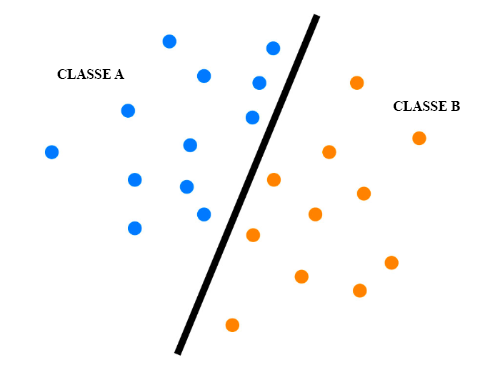
\includegraphics[width=0.8\textwidth]{images/class.png}
        \caption{Esempio di classificazione.}
        \label{fig:rapp_file}
        \end{figure}
    \item \textbf{Regressione:} lo scopo di un modello che effettua regressione è quello di trovare la relazione tra le variabili di input e la variabile di output, che è in questo caso continua. Si cerca quindi l'iperpiano che modella meglio i dati. Durante l'addestramento si modificano i coefficienti dell'equazione che definisce l'iperpiano in modo da minimizzare l'errore.
        \begin{figure}[H]
        \centering
        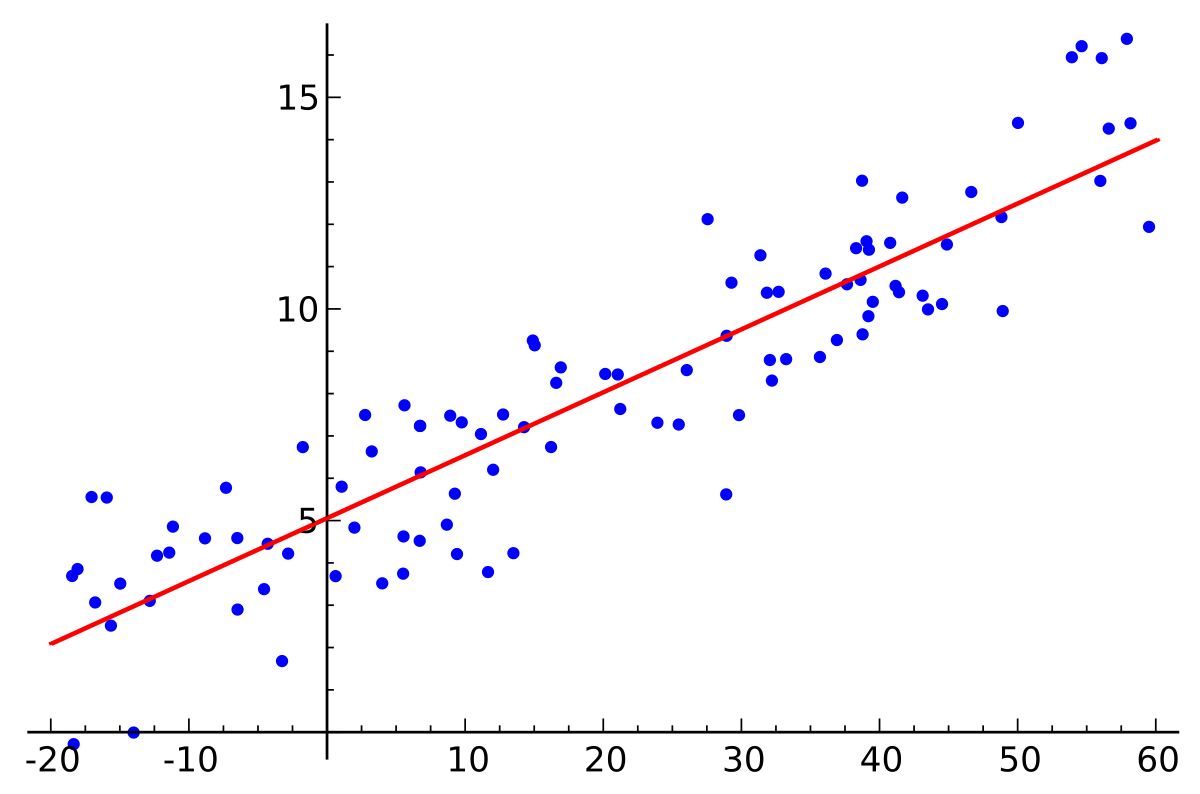
\includegraphics[width=0.8\textwidth]{images/regressione.png}
        \caption{Esempio di regressione.}
        \label{fig:rapp_file}
        \end{figure}
    \item \textbf{Clustering:} consiste nella divisione di oggetti in gruppi non noti a priori, ma che vengono creati unendo gli input simili tra loro e separando quelli con caratteristiche diverse. Dato che le classi non sono note a priori, solitamente per il clustering viene utilizzato un apprendimento non supervisionato.
        \begin{figure}[H]
        \centering
        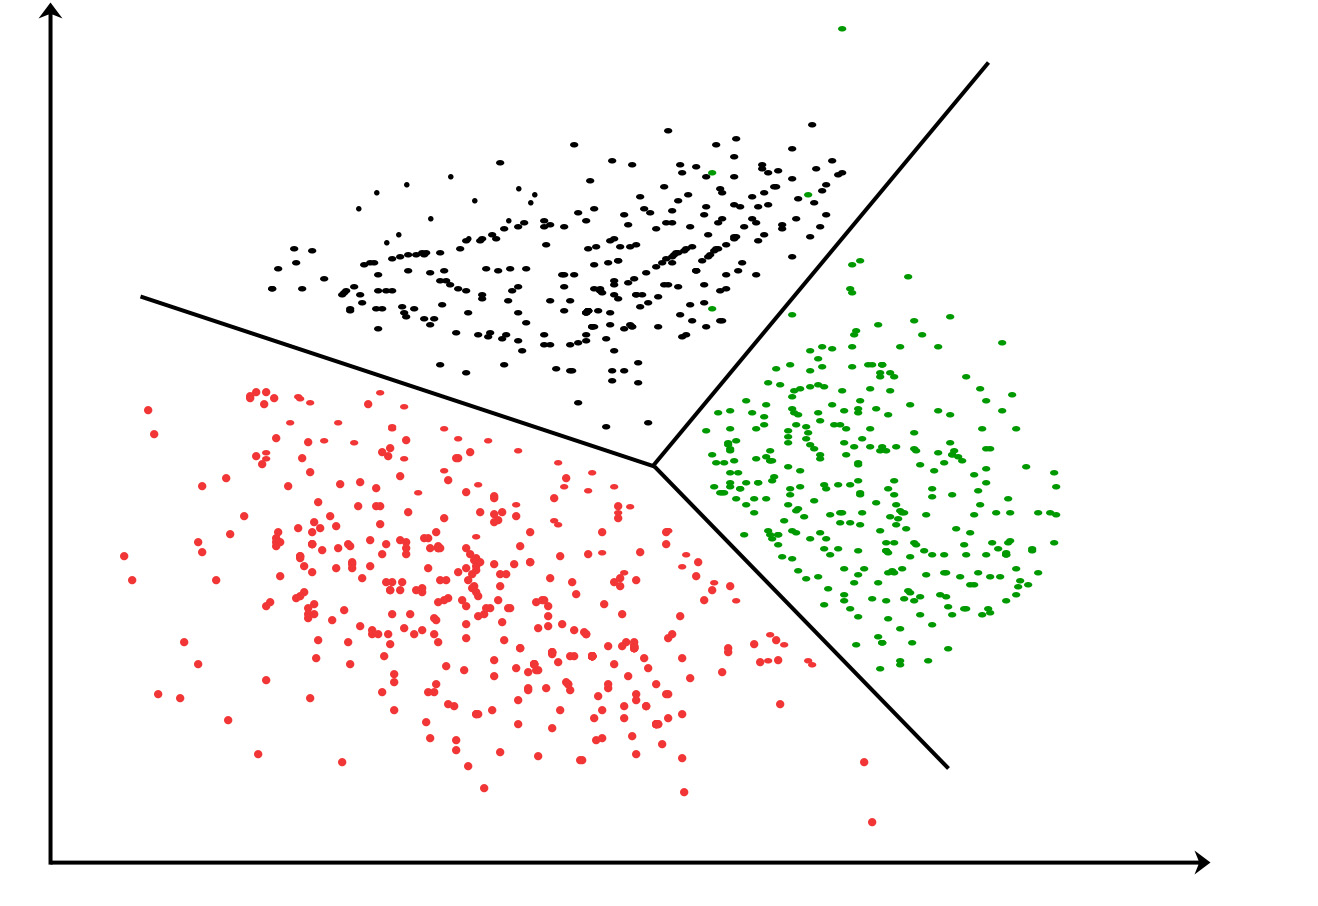
\includegraphics[width=0.8\textwidth]{images/clustering.jpg}
        \caption{Esempio di clustering.}
        \label{fig:rapp_file}
        \end{figure}
\end{itemize}


\section{Reti Neurali}

Le reti neurali sono un modello computazionale costituito da molteplici strati di nodi elementari. La prima rete neurale viene proposta da Rosenblatt nel 1958: il Perceptron. 
L’elemento base delle reti neurali è quindi il “neurone”. 

\begin{figure}[H]
\centering
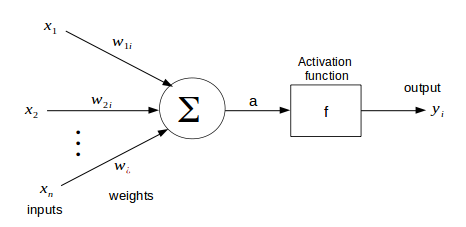
\includegraphics[width=0.8\textwidth]{images/neurone.png}
\caption{Unità neuronale.}
\label{fig:rapp_file}
\end{figure}

Ogni neurone è in pratica un modello di regressione. Può avere uno o più input a ciascuno dei quali è associato un peso, che stabilisce quanto l’input corrispondente influisce sul risultato finale. Prima dell’output è applicata una funzione di attivazione, che stabilisce se l’output del neurone sarà attivo o no. Queste funzioni di attivazione determinano il valore del segnale in uscita in base alla somma dei valori in ingresso moltiplicati per i relativi pesi.

Esistono diversi tipi di funzioni di attivazione, ciascuna delle quali modella l’output del neurone in maniera diversa. 
Alcune funzioni di attivazione sono le seguenti:
\begin{itemize}
    \item \textbf{Linear:} La funzione di attivazione lineare non modifica in alcun modo l’output del nodo, che corrisponderà quindi alla somma di ogni input moltiplicato per il relativo peso. La sua equazione corrisponde a F(x)=x
    
    \begin{figure}[H]
    \centering
    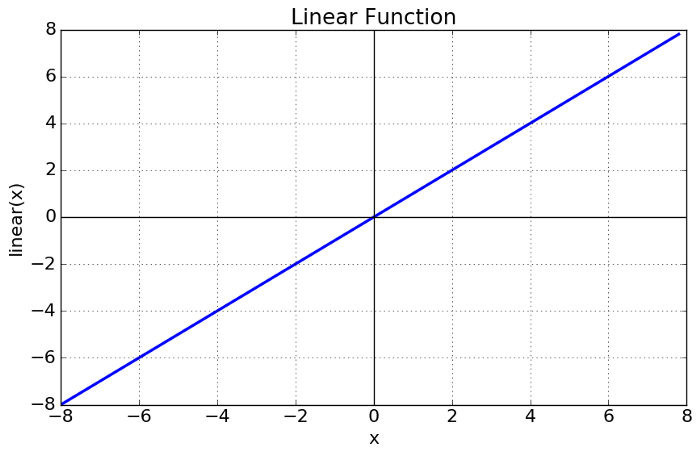
\includegraphics[width=0.8\textwidth]{images/linear.png}
    \caption{Funzione di attivazione lineare.}
    \label{fig:rapp_file}
    \end{figure}
    
    \item \textbf{ReLu:} La funzione di attivazione ReLu (Rectified Linear Unit) è una delle funzioni di attivazione più usate. È definita dalla seguente funzione: 
    \begin{math}
        F\left ( x \right ) = max\left ( 0,x \right )
    \end{math}
   
    
    \begin{figure}[H]
    \centering
    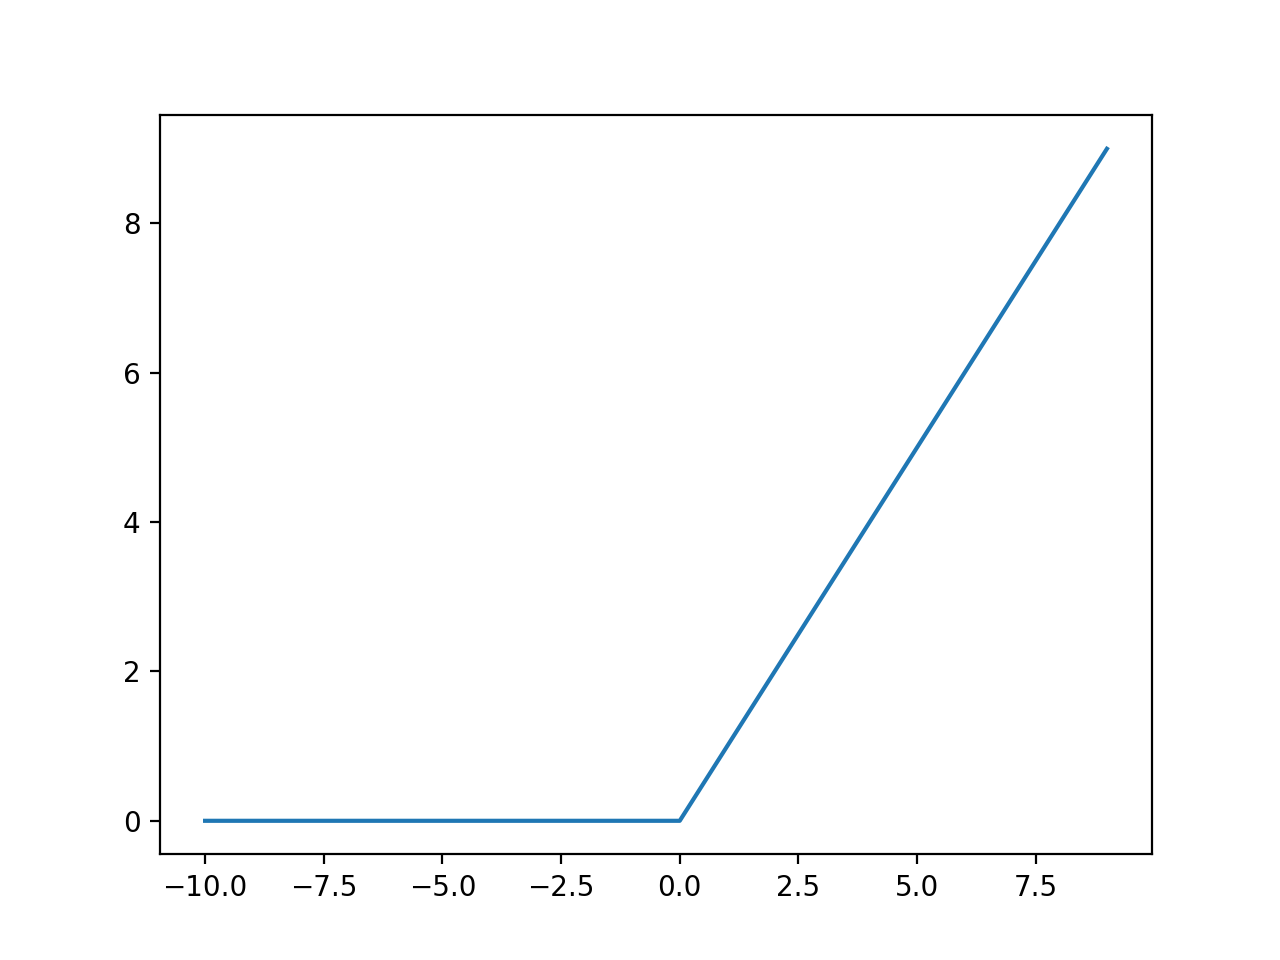
\includegraphics[width=0.8\textwidth]{images/ReLU.png}
    \caption{Funzione di attivazione ReLu.}
    \label{fig:rapp_file}
    \end{figure}
    
    \item \textbf{Softmax:} Questa funzione comprime gli input in modo che la somma dei valori valga 1, mantenendo però le proporzioni originali. È ampiamente utilizzata nell’output layer delle reti neurali che effettuano classificazione.
\end{itemize}

Una rete neurale è composta da un numero arbitrario di questi nodi, raggruppati in livelli detti layer. Ogni rete ha un layer di input e uno di output, tra questi, ci possono essere uno o più hidden layer (layer nascosto). L’output di ogni livello sarà l’input di quello successivo. Il numero di layer nascosti è deciso in fase progettuale. La figura 1.7 mostra un esempio di rete neurale feed forward, dove i dati vanno sempre nella stessa direzione, ovvero dal layer di input verso quello di output.

\begin{figure}[H]
\centering
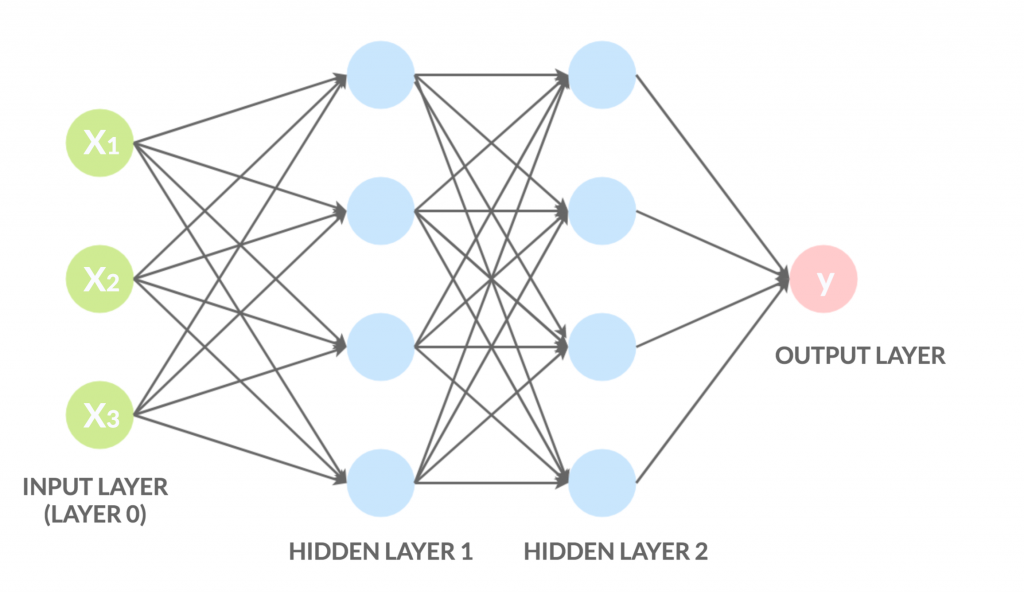
\includegraphics[width=0.8\textwidth]{images/neuralnetwork.png}
\caption{Rete neurale feed forward.}
\label{fig:rapp_file}
\end{figure}


\subsection{Discesa del gradiente}
La discesa del gradiente\cite{DBLP:conf/icnn/Lewis88} è un metodo iterativo per trovare un punto di minimo di una funzione utilizzando appunto il suo gradiente.
Il gradiente è il vettore delle derivate parziali di una funzione per ciascuna delle sue variabili. Calcolando il gradiente in un punto della funzione sapremo l'inclinazione della curva in quel punto e in che direzione si trova un punto di minimo locale.
La discesa del gradiente calcola quindi il gradiente in un punto della curva e gli sottrae un vettore proporzionale, trovando un nuovo punto. Questa operazione viene eseguita più e più volte fino a quando non si converge ad un punto di minimo locale.
Un iperparametro importante in questo algoritmo è in learning rate, che indica la lunghezza del passo nella discesa del gradiente. Se è troppo alto si rischia di "saltare" il punto di minimo, se troppo basso l'algoritmo impiega troppo tempo a convergere.
La funzione su cui si effettua la discesa del gradiente è la funzione di errore. Trovare un punto di minimo in questa funzione equivale a trovare i coefficienti per i quali la funzione approssima meglio i dati.

\begin{figure}[H]
\centering
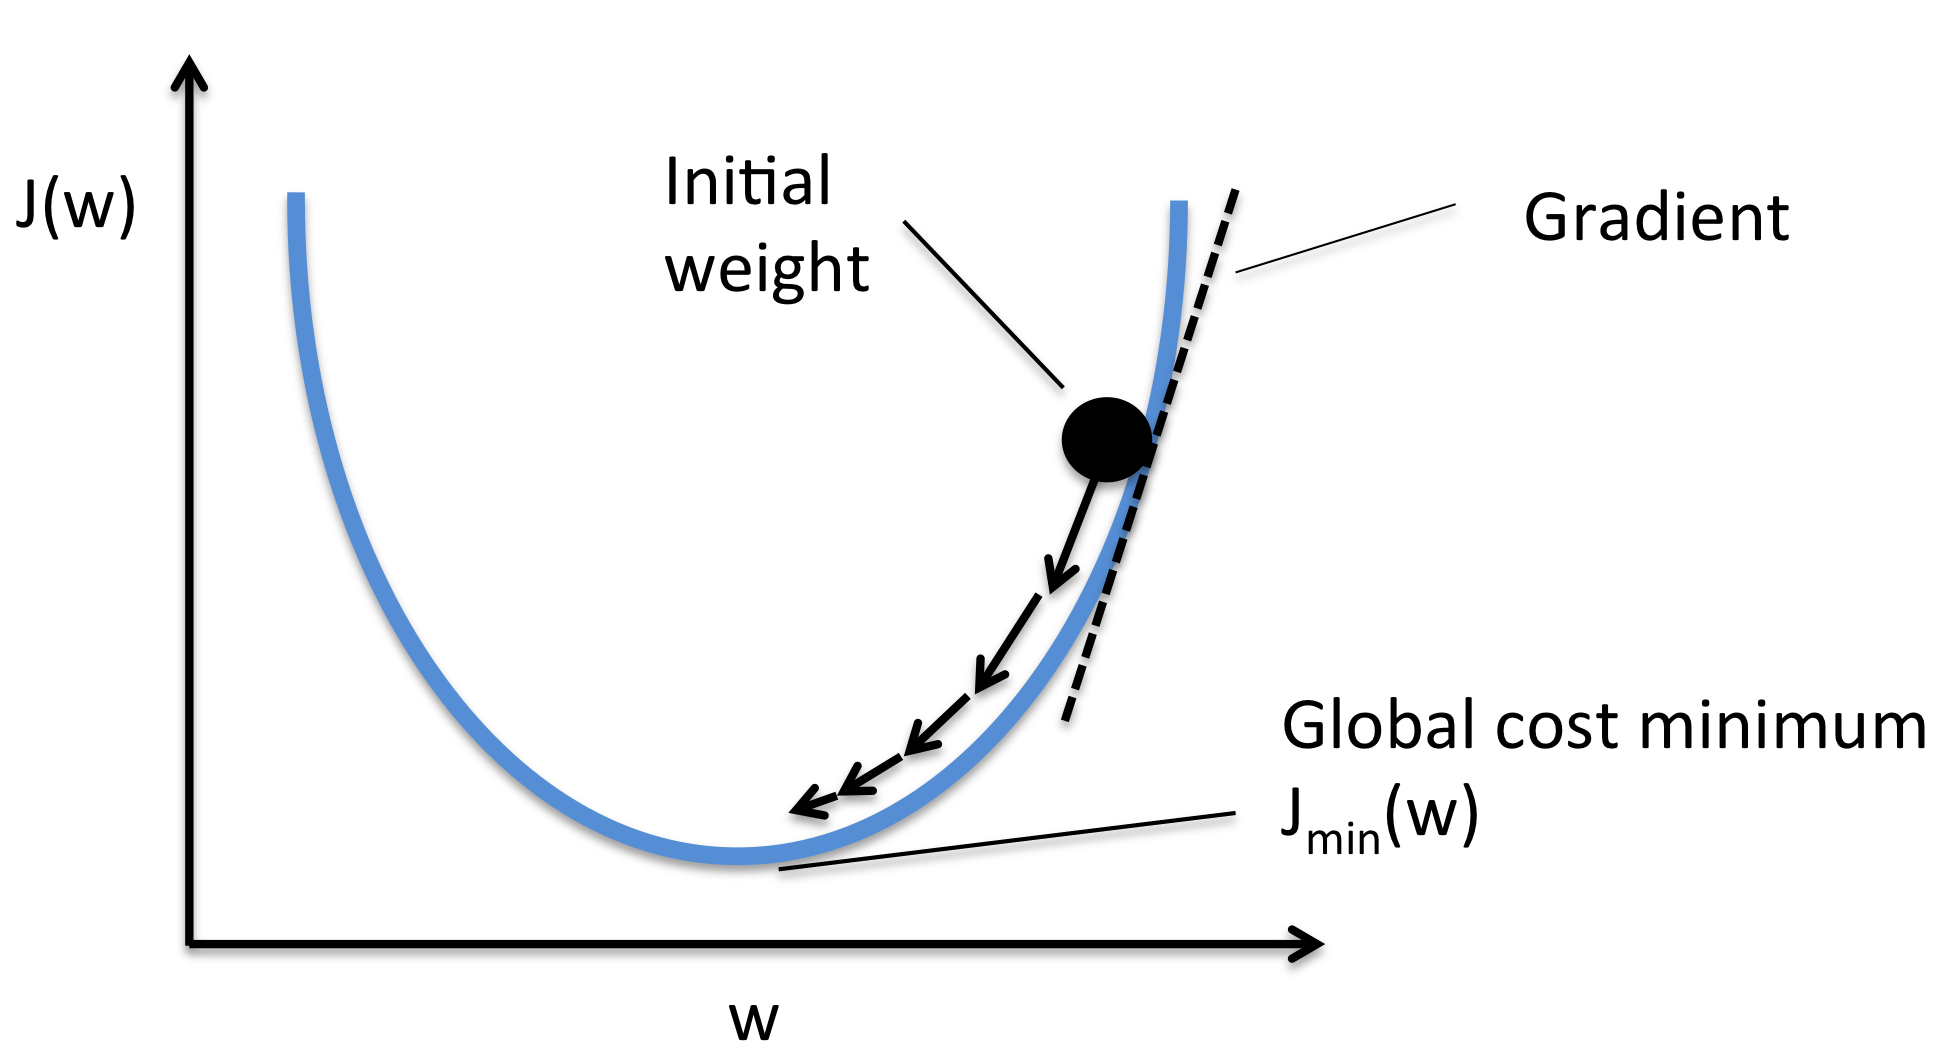
\includegraphics[width=0.8\textwidth]{images/gradient.png}
\caption{Discesa del gradiente.}
\label{fig:rapp_file}
\end{figure}

\section{Time embeddings}

In ogni problema che comprenda le serie temporali, il tempo è una delle feature più importanti. Lo è anche nel caso della predizione di un indice di borsa.
Nel paper “Time2Vec: Learning a Vector Representation of Time”\cite{DBLP:journals/corr/abs-1907-05321} gli autori propongono una soluzione per rappresentare il tempo tramite un vettore. I tre obiettivi alla base della loro ricerca sono di creare una rappresentazione che sia:

\begin{itemize}
    \item \textbf{Semplice:} in modo che possa essere combinata con diversi tipi di modelli. Una matrice, ad esempio, potrebbe risultare difficile da utilizzare in certi casi.
    \item \textbf{Non dipendente dalla scala usata:} il tempo può essere misurato in diversi modi (ore, giorni, minuti...). La rappresentazione non dovrà dipendere dalla scala utilizzata ma essere generica.
    \item \textbf{Periodicità:} la rappresentazione deve essere in grado di catturare sia pattern periodici che non.
\end{itemize}

La definizione matematica di tempo trovata è la seguente:\\

\begin{math}
t2v(t)[i] = \begin{cases}
w_{i}t + l_{i} & \text{ if } i=0 \\ 
F\left ( w_{i}t + l_{i} \right ) & \text{ if } 1\leq i\leq k 
\end{cases}\\
\end{math}
\\
La prima equazione modella eventi temporali non periodici, mentre la seconda si occupa di pattern periodici. Un esempio di pattern periodico è la temperatura che varia nel corso dell’anno, mentre un evento non periodico può essere una malattia, che ha più probabilità di comparire più il paziente è anziano. 
Nell’equazione per modellare i pattern periodici ‘F’ è una funzione di attivazione periodica: dopo vari test effettuati, è emerso che la funzione che ottiene risultati migliori è la funzione seno.

\section{Attention Mechanism}
L’attention\cite{DBLP:conf/nips/VaswaniSPUJGKP17} è una tecnica utilizzata nell’ambito del machine learning che aiuta il modello a concentrarsi solo sugli input rilevanti tra loro, tralasciando gli altri.
\subsection{Single-head e Multi-head attention}
Un'attention head è composta da tre input: Query, Key, Value, ciascuno dei quali riceve una trasformazione lineare. I pesi dell’attention vengono calcolati facendo il prodotto scalare della matrice Query con la matrice Key (K viene trasposta per permettere il calcolo). Gli attention weights vengono poi divisi per la radice della dimensione dei vettori key, in modo da stabilizzare il gradiente durante l’addestramento. I pesi vengono  passati alla funzione softmax che normalizza i pesi in modo che la loro somma sia 1. La matrice ottenuta viene moltiplicata per la matrice Value trasformata e si ottengono gli attention weights finali.
 Il meccanismo di attention può essere riassunto utilizzando la seguente formula:

\begin{math}
\\
Attention\left ( Q,V,K \right ) = softmax\left ( \frac{QK^{T}}{\sqrt{d_{k}}} \right ) V
\end{math}
\\

Ogni attention head da importanza agli input rilevanti tra loro. Utilizzando molteplici attention head è possibile catturare diversi tipi di rilevanza tra i dati. Un multi-head attention layer non fa altro che concatenare gli output di diverse single-head attention.

\section{Transformer}

Il Transformer è un modello di deep learning introdotto nel 2017 e utilizzato principalmente nel campo del Natural Language Processing ma che ha trovato spazio anche in applicazioni di altro genere, come la predizione di serie temporali. I transformer sono progettati per maneggiare dati sequenziali, come le serie temporali.
La sua architettura è composta da un encoder layer che incorpora un meccanismo di self-attention\cite{DBLP:conf/emnlp/TangMRS18} e una rete feed-forward.
Nella versione vanilla del trasformer, l’encoder è seguito da un decoder layer. In questa tesi il decoder non sarà utilizzato in quanto nel nostro caso non è necessario. L’architettura del nostro modello sarà quindi più simile a BERT\cite{DBLP:journals/corr/abs-1810-04805}.
%
% CAPITOLO 2 - MODELLAZIONE DEL PROGETTO
%
\chapter{Modellazione del progetto}
\section{Analisi del dataset}
Il dataset utilizzato è stato ottenuto dal sito 'Yahoo! Finance' direttamente dal codice python utilizzando una libreria apposita.
'yfinance' è una libreria che permette di ottenere degli storici dei dati di mercato relativi a vari indici e titoli di borsa esistenti.
Dopo aver effettuato l’import della libreria, per utilizzarla è necessario creare un oggetto Ticker passandogli, al momento della dichiarazione, il codice relativo all’indice azionario di cui si vogliono ottenere i dati.
I dati su cui è stata svolta questa tesi sono i valori storici dell’indice SP500, che corrisponde al codice “\^GSPC”.
Dopo la creazione del Ticker è sufficiente chiamare il metodo history() per ottenere un Dataframe con i dati. Alla chiamata della funzione è possibile specificare alcuni parametri come il periodo di cui vogliamo avere i dati.

\begin{Verbatim}[commandchars=\\\{\}]
\PY{k+kn}{import} \PY{n+nn}{yfinance}
\PY{n}{sp500} \PY{o}{=} \PY{n}{yfinance}\PY{o}{.}\PY{n}{Ticker}\PY{p}{(}\PY{l+s+s2}{\PYZdq{}}\PY{l+s+s2}{\PYZca{}GSPC}\PY{l+s+s2}{\PYZdq{}}\PY{p}{)}
\PY{n}{data} \PY{o}{=} \PY{n}{sp500}\PY{o}{.}\PY{n}{history}\PY{p}{(}\PY{n}{start}\PY{o}{=}\PY{l+s+s2}{\PYZdq{}}\PY{l+s+s2}{1985\PYZhy{}01\PYZhy{}01}\PY{l+s+s2}{\PYZdq{}}\PY{p}{,} \PY{n}{end}\PY{o}{=}\PY{l+s+s2}{\PYZdq{}}\PY{l+s+s2}{2020\PYZhy{}12\PYZhy{}31}\PY{l+s+s2}{\PYZdq{}}\PY{p}{)}
\end{Verbatim}

In questo elaborato sono stati utilizzati i valori dal 1° gennaio 1985 al 31 dicembre 2020.
\begin{figure}[H]
\centering
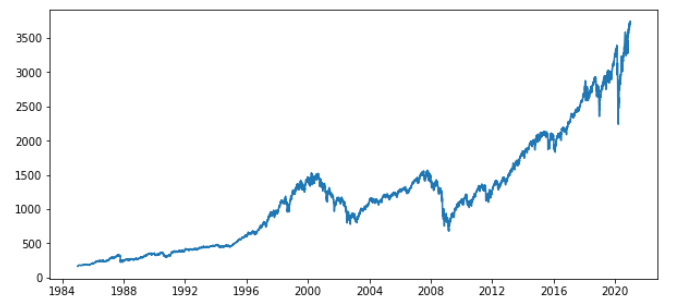
\includegraphics[width=0.8\textwidth]{images/sp500.png}
\caption{Andamento del valore di chiusura dell'indice SP500.}
\label{fig:rapp_file}
\end{figure}

\begin{figure}[H]
\centering
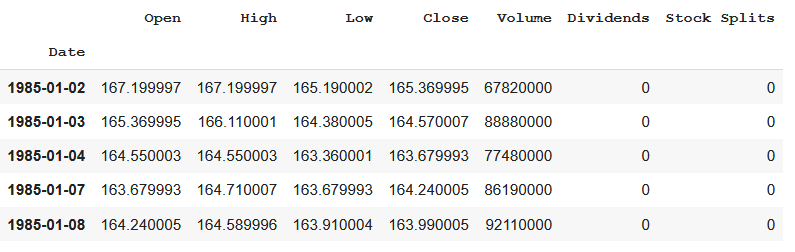
\includegraphics[width=0.8\textwidth]{images/data1.png}
\caption{Le prime cinque righe del dataset.}
\label{fig:rapp_file}
\end{figure}

Come si può notare nella figura 2.2, non tutti i giorni sono presenti, il motivo non è la mancanza di dati nel dataset ma il fatto che la borsa è rimasta chiusa quei giorni.

Ecco la spiegazione delle colonne più significative del dataset:
\begin{itemize}
    \item \textbf{Date:} il giorno di riferimento.
    \item \textbf{Open:} il valore del titolo all’apertura della borsa.
    \item \textbf{High:} il valore più alto raggiunto durante la giornata.
    \item \textbf{Low:} il valore più basso raggiunto durante la giornata.
    \item \textbf{Close:} il valore di chiusura del titolo.
    \item \textbf{Volume:} il numero di transazioni effettuate.
\end{itemize}
\section{Definizione delle classi}
In questo capitolo verrà analizzata nel dettaglio l'architettura delle classi utilizzate
\subsection{Time2Vec}
La prima classe che è stata definita è Time2Vector, ovvero il layer che permette il time embedding. La sua architettura è illustrata nella figura 2.3. I diagrammi che illustrano l'architettura delle classi sono stati creati utilizzando come esempio un modello a cui vengono fornite in input sequenze di 128 giorni e aventi batch size pari a 32.

\begin{figure}[H]
\centering
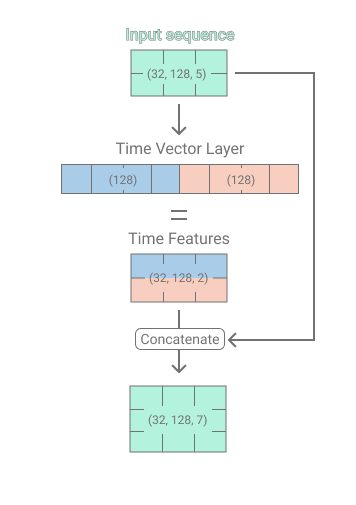
\includegraphics[width=0.8\textwidth]{images/time2vector.png}
\caption{Architettura della classe Time2Vec.}
\label{fig:rapp_file}
\end{figure}

Per ognuna delle 32 sequenze di input e per ciascuno dei 128 giorni, la classe Time2Vector estrarrà le feature temporali periodiche e non periodiche. Otterremo quindi in output due matrici di dimensione (32, 128) contenenti i pesi delle time features.
Prima di essere passato al layer successivo, l’output del Time2Vector viene unito all’input iniziale, in modo che oltre alle time features vengano utilizzati anche i dati originali.


\subsection{SingleAttention}

Utilizzando la teoria dell’attention mechanism, è stata creata la classe SingleAttention. Questa classe è un layer che prende in input l’uscita del Time2Vector e la processa, calcolando gli attention weights.
I tre input (Query, Key, Value), vengono trasformati utilizzando un Dense layer. La dimensione di questo layer è una scelta progettuale ed è fissata a 96.

\begin{figure}[H]
\centering
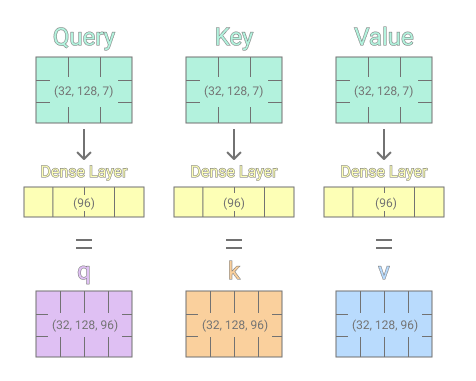
\includegraphics[width=0.8\textwidth]{images/singlehead.png}
\caption{Trasformazione degli input della classe SingleAttention.}
\label{fig:rapp_file}
\end{figure}

A questo punto bisogna per calcolare i pesi dell’attention si procederà come descritto in precedenza: viene calcolato il prodotto scalare tra Q e K (K viene trasposta per permettere il calcolo). Il risultato viene diviso per la radice della dimensione del Dense Layer, che corrisponde a 96. E' poi applicata la funzione softmax e infine viene eseguita la moltiplicazione per la matrice V.
Questa seconda parte della classe ha quindi la seguente architettura:

\begin{figure}[H]
\centering
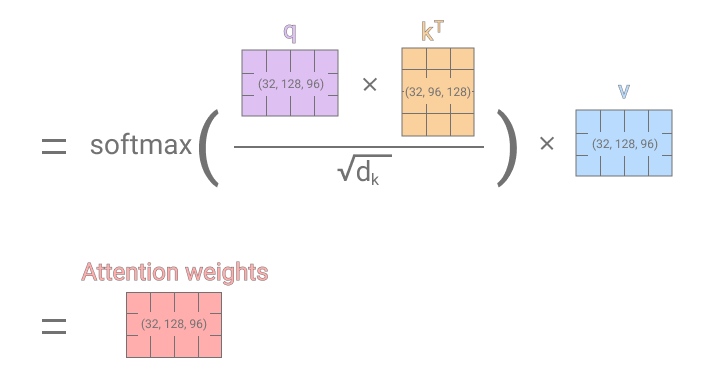
\includegraphics[width=0.8\textwidth]{images/single2.png}
\caption{Calcolo degli attention weights.}
\label{fig:rapp_file}
\end{figure}

\subsection{MultiAttention}

La classe MultiAttention riceve in input gli attention weights delle singole head attention. Questi input sono concatenati e poi trasformati utilizzandoo un Dense layer di dimensione 7, in modo da riportare la matrice alla stessa dimensione di quella in output al Time2Vector.
Rispetto alle altre questa classe ha un’architettura più semplice e al suo interno non vengono effettuate operazioni complesse.


\begin{figure}[H]
\centering
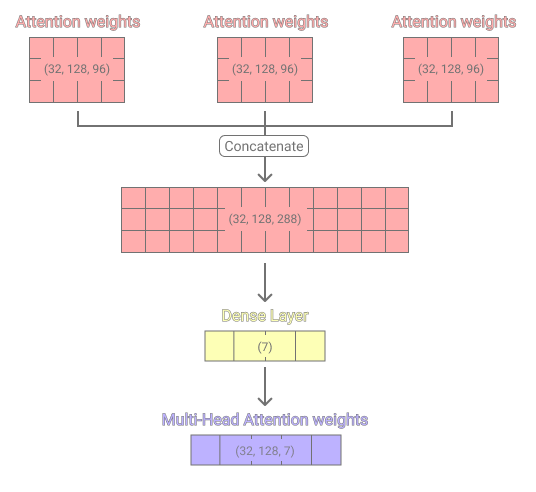
\includegraphics[width=0.8\textwidth]{images/multi.png}
\caption{Architettura della classe MultiAttention.}
\label{fig:rapp_file}
\end{figure}

\subsection{TransformerEncoder}

La classe TransformerEncoder implementa una versione custom del Transformer, che prevede solamente l’encoder ma non il decoder. Come nell’architettura originale l’encoder è formato da due parti: un meccanismo di attention e una rete feed forward.
La rete feed forward è stata creata utilizzando due Dense layer: il primo di dimensione 256 e funzione di attivazione ReLu, il secondo di dimensione 7.
È inoltre presente un Dropout layer, la cui funzione è quella di prevenire l’overfitting del modello disattivando alcuni neuroni ad ogni step di training.
L’output del layer di dropout viene sommato all’input originale (Output della classe Time2Vector). 
L’aggiunta di un normalization layer garantisce che ogni feature venga normalizzata (Valore medio 0 e varianza 1) e aiuta a ridurre l’overfitting.
La combinazione dei layer: Dropout, somma dell’input originale e normalizzazione è presente sia dopo il meccanismo di attention che dopo la rete feed forward.

\begin{figure}[H]
\centering
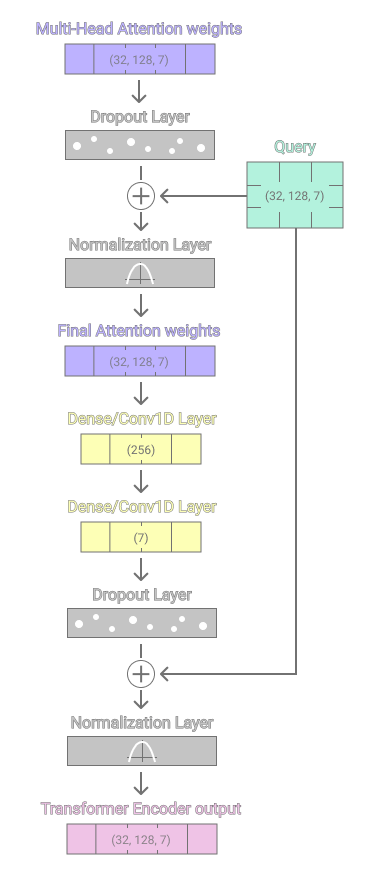
\includegraphics[width=0.6\textwidth]{images/transformer.png}
\caption{Architettura della classe TransformerEncoder.}
\label{fig:rapp_file}
\end{figure}

%
% CAPITOLO 3 - SVILUPPO DELL'APPLICAZIONE
%

\chapter{Sviluppo dell'applicazione}

\section{Preprocessamento dei dati}

In questa sezione verranno illustrate le operazioni effettuate sul dataset prima di fornirli al modello per l'addestramento.

\subsection{Operazioni preliminari e standardizzazione}
Prima di utilizzare i dati, occorre fare alcune modifiche al fine di renderli ottimali per l’addestramento della rete. Questa fase si chiama pre-processing dei dati.
Per prima cosa sono state rimosse le colonne “Dividens” e “Stock Splits” in quanto non contengono informazioni utili alla predizione del valore di chiusura.

La predizione del valore di un indice di borsa può essere affrontata sia come un problema di regressione che di classificazione. In questo elaborato è stato trattato come una classificazione, occorre quindi assegnare ad ogni giorno una classe. Se il valore di chiusura di un giorno sarà superiore al valore di apertura significa che l’indice è salito e gli sarà assegnata la classe 1. Al contrario se il valore di chiusura è sceso rispetto a quello di apertura avrà classe 0. Queste classi vengono assegnate aggiungendo una colonna al dataframe originale.

Addestrando il modello utilizzando il valore assoluto del titolo si rischia di non riuscire a cogliere le piccole variazioni del titolo. I dati sono stati quindi modificati in modo che ogni valore sia il cambiamento in percentuale del valore del titolo rispetto al giorno precedente.

Successivamente è stata effettuata la standardizzazione dei dati, ovvero modificati in modo che abbiano una distribuzione gaussiana di media 0 e varianza 1.
La standardizzazione è ampiamente utilizzata nell’ambito del machine learning in quanto ha effetti positivi sull’addestramento dei modelli ed è particolarmente efficace se i dati originali hanno scale diverse tra loro.

\begin{figure}[H]
\centering
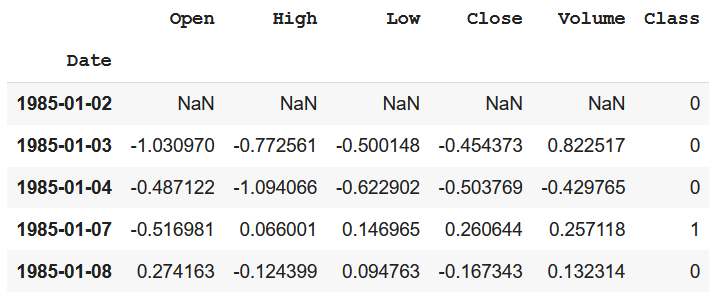
\includegraphics[width=0.6\textwidth]{images/data2.png}
\caption{Alcune istanze del dataset dopo le prime operazioni di pre-processing.}
\label{fig:rapp_file}
\end{figure}

\begin{figure}[H]
\centering
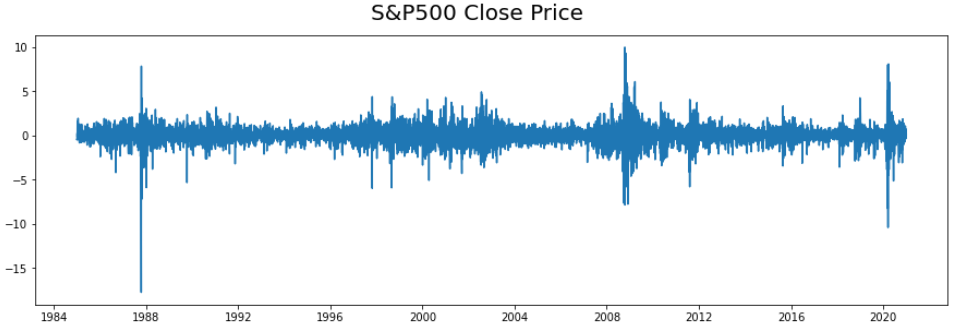
\includegraphics[width=0.6\textwidth]{images/data3.png}
\caption{Grafico dei dati.}
\label{fig:rapp_file}
\end{figure}

\subsection{Divisione dei dati}
Per addestrare e valutare il modello occorre dividere i dati in Training, Validation e Test set. Il training set viene utilizzato per addestrare la rete, il validation set per fare il tuning degli iperparametri e il test set per valutare il modello su dati “nuovi”.
Esistono in letteratura diversi metodi per suddividere i dati. In questa tesi è stata utilizzata la cross fold validation. Questa tecnica consiste nel dividere i dati in k fold: ogni addestramento viene effettuato utilizzando una fold come validation set e le restanti come training set. Per ogni training si misurano le performance del modello e si effettuerà la media di queste per ottenere la valutazione finale del modello.

\begin{figure}[H]
\centering
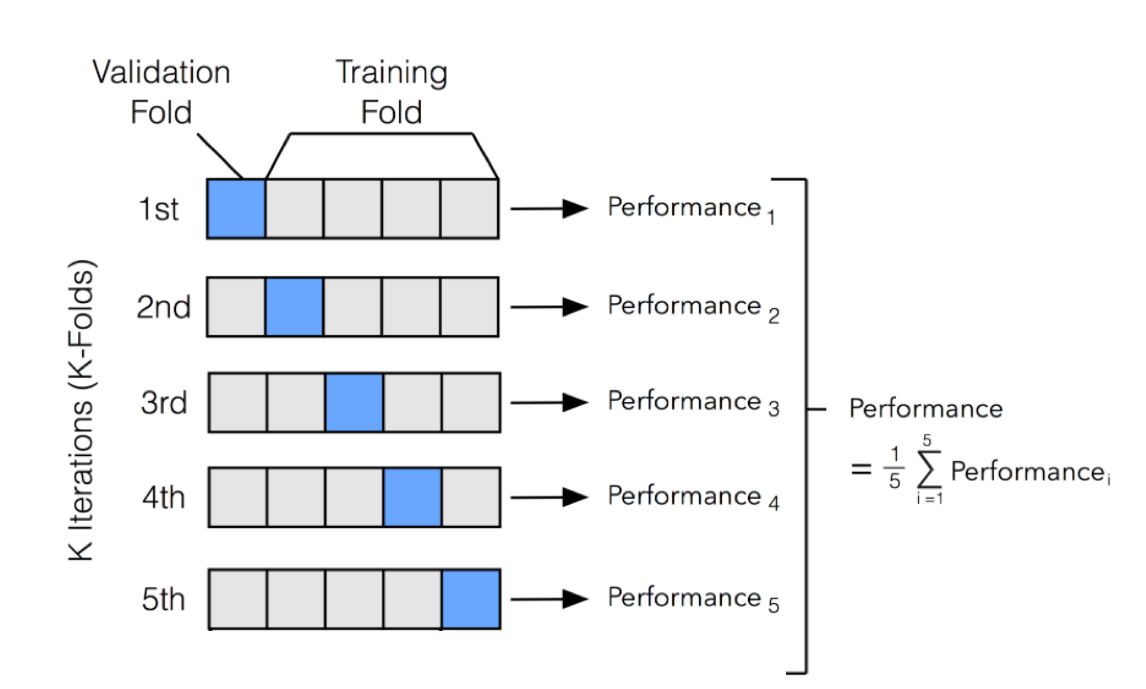
\includegraphics[width=0.6\textwidth]{images/kfolds.png}
\caption{Cross-fold validation.}
\label{fig:rapp_file}
\end{figure}

Per la predizione di serie temporali non è però possibile utilizzare la cross fold validation, dato che si andrebbero a predire valori passati utilizzando quelli futuri.
Nella figura 3.4 è illustrato come viene modificata questa tecnica in modo che sia compatibile con le serie temporali.
Ad ogni iterazione un certo numero di dati non viene utilizzato e per l’addestramento vengo utilizzati solo dati precedenti a quelli che compongono il test set. La performance del modello viene calcolata come la media delle performance delle varie iterazioni.
https://www.overleaf.com/project/5ed943b9487c28000198567a
\begin{figure}[H]
\centering
\includegraphics[width=0.6\textwidth]{images/timesplit.png}
\caption{Cross-fold validation adattata alle serie temporali.}
\label{fig:rapp_file}
\end{figure}

\subsection{Creazione delle sequenze di input}
L’obiettivo del modello è quello di predire il valore di chiusura di un determinato giorno. Per predire questo valore serve dare in input al modello la sequenza dei giorni precedenti a quello che vogliamo predire.
Per questo motivo sono state create delle sotto sequenze di un certo numero di giorni, la cui lunghezza è un parametro del modello.


\begin{Verbatim}[commandchars=\\\{\}]
\PY{k}{def} \PY{n+nf}{create\PYZus{}sequence}\PY{p}{(}\PY{n}{data}\PY{p}{)}\PY{p}{:}
  \PY{n}{X}\PY{p}{,} \PY{n}{y} \PY{o}{=} \PY{p}{[}\PY{p}{]}\PY{p}{,} \PY{p}{[}\PY{p}{]}
  \PY{k}{for} \PY{n}{i} \PY{o+ow}{in} \PY{n+nb}{range}\PY{p}{(}\PY{n}{seq\PYZus{}len}\PY{p}{,} \PY{n+nb}{len}\PY{p}{(}\PY{n}{data}\PY{p}{)}\PY{o}{\PYZhy{}}\PY{l+m+mi}{1}\PY{p}{)}\PY{p}{:}
    \PY{n}{X}\PY{o}{.}\PY{n}{append}\PY{p}{(}\PY{n}{data}\PY{p}{[}\PY{p}{:}\PY{p}{,} \PY{p}{:}\PY{l+m+mi}{5}\PY{p}{]}\PY{p}{[}\PY{n}{i}\PY{o}{\PYZhy{}}\PY{n}{seq\PYZus{}len}\PY{p}{:}\PY{n}{i}\PY{p}{]}\PY{p}{)}
    \PY{n}{y}\PY{o}{.}\PY{n}{append}\PY{p}{(}\PY{n}{data}\PY{p}{[}\PY{p}{:}\PY{p}{,} \PY{l+m+mi}{5}\PY{p}{]}\PY{p}{[}\PY{n}{i}\PY{p}{]}\PY{p}{)}
  \PY{n}{X}\PY{p}{,} \PY{n}{y} \PY{o}{=} \PY{n}{np}\PY{o}{.}\PY{n}{array}\PY{p}{(}\PY{n}{X}\PY{p}{)}\PY{p}{,} \PY{n}{np}\PY{o}{.}\PY{n}{array}\PY{p}{(}\PY{n}{y}\PY{p}{)}
  \PY{n}{y} \PY{o}{=} \PY{n}{to\PYZus{}categorical}\PY{p}{(}\PY{n}{y}\PY{p}{)}
  \PY{k}{return} \PY{n}{X}\PY{p}{,} \PY{n}{y}
\end{Verbatim}



\section{Creazione del modello}
\begin{figure}[H]
\centering
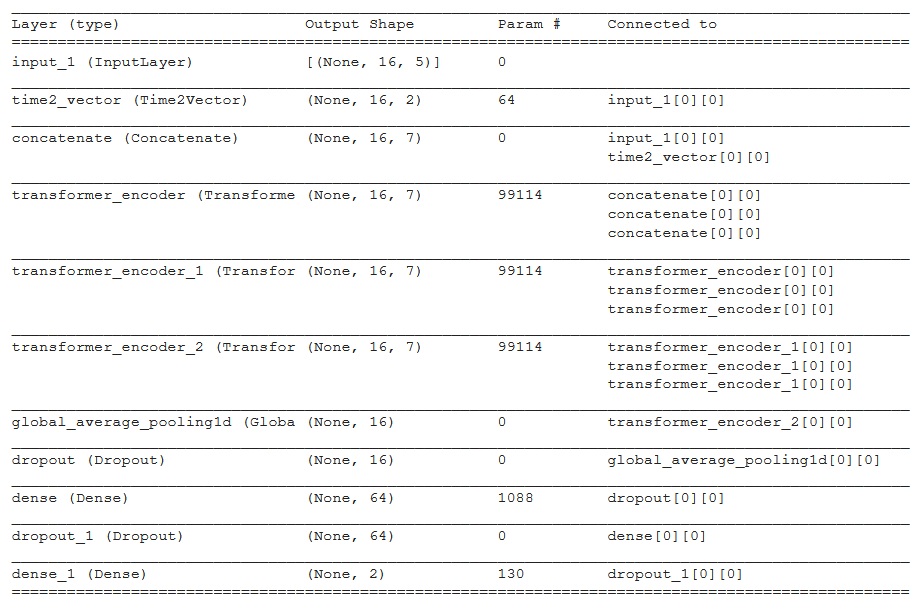
\includegraphics[width=1\textwidth]{images/model.png}
\caption{Architettura finale del modello.}
\label{fig:rapp_file}
\end{figure}
Come si può vedere nella figura 3.5 sono stati utilizzati tre TransformerEncoder in cascata.
Dopo l’ultimo transformer è presente un layer GlobalAveragePooling1D: la funzione di questo layer è di ridurre di una dimensione le features.
Successivamente è presente un dropout layer seguito da un Dense layer di dimensione 64 e funzione di attivazione ReLu.
Infine, è stato inserito un altro dropout layer prima dell’output layer.
Il layer di uscita è un Dense layer di dimensione 2 (un nodo per classe) e funzione di attivazione Softmax. Questo layer effettua quindi una classificazione a due classi. Nel caso si voglia cambiare il tipo di predizione e passare ad esempio da una classificazione ad una regressione è sufficiente modificare quest'ultimo layer.

\section{Addestramento}
Per l’addestramento della rete, è stata utilizzata una versione della cross-fold validation adattata alla gestione di serie temporali. Sono stati personalizzati i seguenti parametri del training:
\begin{itemize}
    \item \textbf{Epoca:} è il numero di iterazioni complete sul training set che il modello effettua durante l’addestramento. Il numero di epoche è deciso a seconda della complessità del problema, della grandezza del training set e altri fattori. Se durante l’addestramento l’accuratezza del modello non migliora col passare delle epoche è possibile che la funzione d’errore sia già stata minimizzata e non ha significato continuare l’addestramento
    \item \textbf{Batch size:} è il numero di sequenze di dati di input fornite contemporaneamente al modello durante la fase di training. Avendo utilizzato un batch size di dimensione 32 significa che il modello riceve 32 sequenze di 128 giorni.
    \item \textbf{Loss Function:} la funzione di loss è la funzione da minimizzare durante l’addestramento. È stata utilizzata la
\end{itemize}
Per l’addestramento di una rete neurale è fondamentale utilizzare le callback. Le callback sono funzioni che vengono chiamate al termine di ogni epoca di training e possono fornire diverse informazioni utili. Durante l’addestramento è stata utilizzata principalmente la callback ModelCheckpoint(). Questa funzione permette di valutare i parametri del modello e nel caso sia migliorato rispetto all’epoca precedente lo salva. In questo modo, al termine dell’addestramento, sarà stato salvato il modello migliore.
L’addestramento è stato fatto monitorando la loss sul validation set, la callback salva quindi il modello quando il valore della loss sul validation raggiunge un nuovo minimo.

\chapter{Risultati ottenuti}
In questo capitolo verranno illustrati i metodi di valutazione, gli esperimenti effettuati e i risultati ottenuti.
\section{Metodo di valutazione}
Definiamo la classe UP come i giorni nei quali il valore dell’indice aumenta rispetto al giorno precedente. Al contrario la classe DOWN sarà composta dai giorni in cui i valori scendono.
Possiamo stampare la matrice di confusione del modello, ovvero la matrice che indica il numero di istanze predette correttamente e non, per ogni classe. Esempio di confusion matrix:

\begin{figure}[H]
\centering
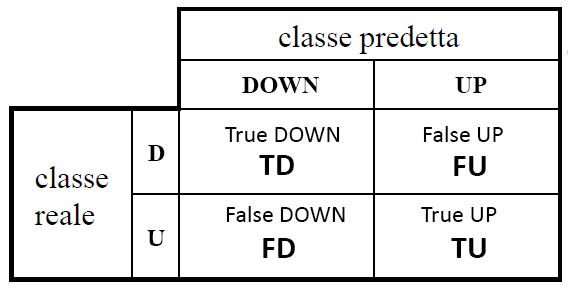
\includegraphics[width=0.6\textwidth]{images/cm2.png}
\caption{Esempio di una matrice di confusione.}
\label{fig:rapp_file}
\end{figure}

Il modello, data una sequenza di giorni in input, divide gli output in base alla loro classe di appartenenza. Per la valutazione di un modello di classificazione esistono diverse metriche:

\begin{itemize}
    \item \textbf{Accuratezza:} è la percentuale di output predetti correttamente, sul totale delle istanze.
	\[Accuracy = \frac{TU+TD}{TU+TD+FU+FD}\]
    \item \textbf{Precisione:}  è la percentuale di output predetti correttamente di una classe.
    \[Precision(a) = \frac{TU}{TU+FU}\]
    \item \textbf{Recall:} data una classe, è la percentuale di predizioni corrette su quella classe.
    \[Recall(a) = \frac{TU}{TU+FD}\]
\end{itemize}

La metrica da utilizzare per la valutazione dipende dal problema, solitamente precision e recall sono utilizzate quando le classi sono sbilanciate. Ipotizziamo di essere in campo medico e voler classificare delle cellule in benigne e maligne. In questo caso vogliamo classificare tutte le cellule maligne come tali, anche a costo di ottenere dei falsi positivi, che possono essere poi analizzati meglio in seguito. Ed è per questo che si utilizza il Recall sulla classe maligne.
Nell’ambito della predizione di un valore di indice di borsa, in generale, è sufficiente utilizzare come metrica l’accuratezza, dato che vogliamo avere più istanze possibili predette correttamente, indipendentemente dalla loro classe di appartenenza.

\section{Esperimenti e risultati}
Gli indici di borsa, racchiudendo al loro interno azioni di molte aziende, tendono tendenzialmente a salire.
Per la valutazione del modello, oltre alle metriche già citate in precedenza, è stato confrontato il modello addestrato con uno che predice sempre la crescita del valore dell'indice.

Nei primi esperimenti effettuati, i dati erano stati suddivisi nei set con metodo hold-out, in particolare veniva utilizzato l'80\% iniziale dei dati come training, il successivo 10\% come validation set e l'ultimo 10\% come test set. Utilizzando questa suddivisione il risultato migliore ottenuto è stata un'accuratezza del 53\% sul test set. 

Per migliorare i risultati i modelli successivi sono stati addestrati con dati suddivisi utilizzando la cross-fold validation adattata alle serie temporali spiegata in precedenza.

Il primo modello è stato addestrato utilizzando i seguenti parametri:
\begin{itemize}
    \item \textbf{Numero di epoche:} 20
    \item \textbf{Numero di validation set:} 6
    \item \textbf{Dimensione validation set:} 20
    \item \textbf{Dimensione del test set:} 40
    \item \textbf{Lunghezza sequenza di input:} 16
    \item \textbf{Numero di attention heads:} 12
    \item \textbf{Batch size:} 64
\end{itemize}

Il modello ha raggiunto un'accuratezza media del 56\% sui validation set. Per fare una valutazione completa è opportuno testare il modello su dati non visti durante l'addestramento, per farlo utilizziamo un test set di 40 giorni. 
I risultati ottenuti sono stati i seguenti:

\begin{figure}[H]
\centering
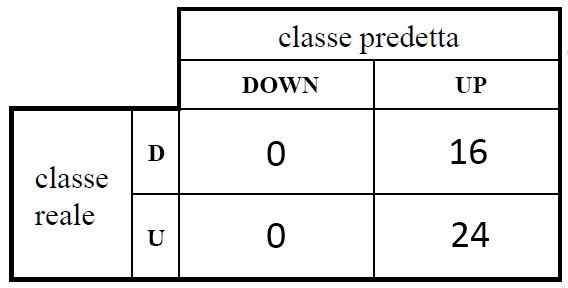
\includegraphics[width=0.6\textwidth]{images/test_1.png}
\caption{Matrice di confusione del modello.}
\label{fig:rapp_file}
\end{figure}

Dalla matrice di confusione è possibile calcolare l'accuratezza del modello sul test set, che è pari al 60\%.
Il modello ha predetto sempre il rialzo del titolo, ha quindi capito l'andamento a lungo termine dell'indice ma non riesce a cogliere le variazioni giornaliere del valore. 
Per superare questo problema è stato addestrato un altro modello, aumentando il numero di epoche di addestramento da 20 a 35.
L'aumento del numero di epoche non ha portato a miglioramenti significativi nei risultati del modello: l'accuratezza media sul validation set è salita a 59\% (3\% in più rispetto al modello precedente) ma l'accuratezza sul test set è rimasta al 60\%.
La matrice di confusione prodotta è uguale alla precedente, il modello predice sempre il rialzo dell'indice.

Il test successivo è stato eseguito con i seguenti parametri:
\begin{itemize}
    \item \textbf{Numero di epoche:} 25
    \item \textbf{Numero di validation set:} 6
    \item \textbf{Dimensione validation set:} 20
    \item \textbf{Dimensione del test set:} 40
    \item \textbf{Lunghezza sequenza di input:} 32
    \item \textbf{Numero di attention heads:} 12
    \item \textbf{Batch size:} 64
\end{itemize}

Per addestrare la rete è stato aumentato il numero di epoche ed è stata raddoppiata la lunghezza delle sequenze di input. Questo significa che la predizione del valore di chiusura viene effettuata utilizzando i 32 giorni precedenti invece dei 16 utilizzati dai modelli visti fino ad ora.
Questo modello ha ottenuto un'accuratezza del 54\% sui validation set (leggermente meno del precedente). E' migliorata l'accuratezza delle predizioni sul test set:

\begin{figure}[H]
\centering
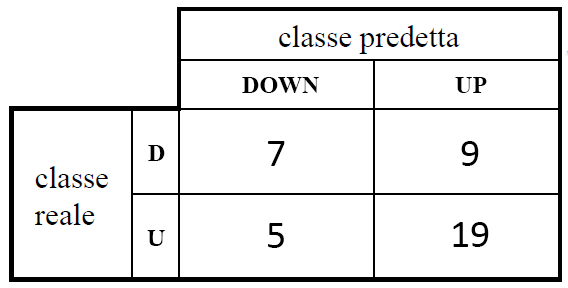
\includegraphics[width=0.6\textwidth]{images/test_2.png}
\caption{Matrice di confusione del modello.}
\label{fig:rapp_file}
\end{figure}

Il modello ha raggiunto un'accuratezza del 65\% su dati nuovi, superando anche l'accuratezza di un modello che predice sempre il rialzo, pari al 60\%.

L'esperimento successivo è stato effettuato aumenta il numero di test e validation set da 6 a 10. Il modello generato non ha ottenuto risultati migliori del precedente: l'accuratezza sul test set è rimasta invariata (65\%) nonostante le differenze nelle predizioni.

\begin{figure}[H]
\centering
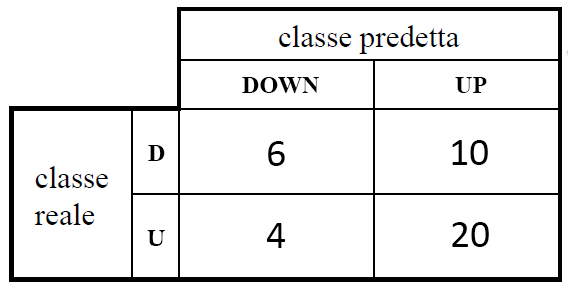
\includegraphics[width=0.6\textwidth]{images/test_3.png}
\caption{Matrice di confusione del modello.}
\label{fig:rapp_file}
\end{figure}

In seguito al miglioramento delle prestazioni dovute all'incremento della lunghezza delle sequenze di input, sono stati addestrati altri due modelli modificando tale parametro.
Il primo, che utilizza sequenze di input di 64 giorni, ha ottenuto un'accuratezza del 60\% sul test set.
Aumentando la dimensione a 128 giorni, è stato notata una diminuzione nelle performance: il modello addestrato ha raggiunto un'accuratezza del 50\% sul test set, molto più bassa delle precedenti.

Da questi esperimenti si conclude che la dimensione ideale per le sequenze di input è tra i 20 e i 40 giorni.

L'accuratezza massima raggiunta, pari al 65\%, è un risultato accettabile data la difficoltà del problema, nonostante sia inferiore a quello che ci si aspettava. 
Le architetture sperimentate hanno dimostrato di poter essere utilizzate anche per la predizione di un indice di borsa, oltre che a risolvere i problemi per cui sono state progettate.


\section{Sviluppi futuri}
Ci sono alcuni aspetti che possono essere migliorati per aumentare l’accuratezza del modello.

Il dataset utilizzato contiene circa 9000 righe. L’aumento delle istanze di training porta grandi benefici al modello, è per questo che l’utilizzo di un dataset di maggiori dimensioni è sicuramente una delle priorità per quanto riguarda lo sviluppo di questo progetto. Per creare questo dataset è necessario utilizzare i dati storici di altri indici che abbiano un comportamento simile allo S\&P500.

Attualmente, il modello riceve come input i dati dei giorni precedenti al giorno del valore di chiusura de predire. Per incrementare le prestazioni si può fornire in input anche il valore di apertura del giorno da predire, valore che è noto ad inizio giornata. Per fare ciò sarà necessario cambiare la struttura dei dati in input e di conseguenza quella della rete.

Attualmente il modello utilizza solamente i dati storici per prevedere l’andamento del valore dell’indice, che è però influenzato da molti altri fattori, come le news e le tendenze. È per questo motivo che ritengo che integrare i dati storici con dati ottenuti attraverso web scraping, possa incrementare l’accuratezza del modello. \cite{DBLP:conf/ic3k/MoroPDPR17} \cite{DBLP:conf/ic3k/DomeniconiMPP17a}

%% RINGRAZIAMENTI
\chapter*{Ringraziamenti}
\addcontentsline{toc}{chapter}{Ringraziamenti}
\markboth{RINGRAZIAMENTI}{RINGRAZIAMENTI}

Vorrei ringraziare il mio relatore, il professor Moro, per avermi fatto appassionare all’ambito della data science e per avermi guidato nello svolgimento di questa tesi.

Grazie alla mia famiglia, che mi ha sempre sostenuto in questi anni e mi ha messo nelle migliori condizioni possibili per terminare questo percorso.


Infine vorrei ringraziare tutti i miei amici e i miei compagni di corso che mi sono stati vicino durante questi anni, ognuno di voi mi ha aiutato a raggiungere questo traguardo.
	
\backmatter	
\addcontentsline{toc}{chapter}{Bibliografia}
\bibliographystyle{unsrt}
% i riferimenti bibliografici, che devono essere almeno 20 per una tesi triennale ed almeno 30 per una della magistrale, si scaricano da qui https://dblp.uni-trier.de/search/
% e si aggiungono al file bibliografia.bib, dopodichè si citano opportuanamente nel testo della tesi con \cite{label}  dove label è il primo elemento di ogni rif. bibliografico subito dopo la parentesi graffa aperta, e.g. DBLP:books/daglib/0087929 (vedi file .bib sopra menzionato)
\bibliography{bibliografia}


\end{document}
